\newpage
\let\cleardoublepage\clearpage
\chapter{Горное и нефтегазовое дело}
МРНТИ 52.13.25
\hfill {\bfseries \href{https://doi.org/10.58805/kazutb.v.3.24-424}{https://doi.org/10.58805/kazutb.v.3.24-424}}

\sectionwithauthors{Д.К. Таханов, М.Ж. Балпанова, Д.Т. Ивадилинова}{ИССЛЕДОВАНИЯ ЗАКОНОМЕРНОСТЕЙ ИЗМЕНЕНИЯ ДЕФОРМАЦИЙ В ЗАВИСИМОСТИ
ОТ ТЕХНОЛОГИЧЕСКИХ ПАРАМЕТРОВ ОЧИСТНОГО ЗАБОЯ ДЛЯ НАКЛОННЫХ ЗАЛЕЖЕЙ}

\begin{center}
{\bfseries \textsuperscript{1}Д.К. Таханов, \textsuperscript{1}М.Ж.
Балпанова\envelope, \textsuperscript{2}Д.Т. Ивадилинова}

\textsuperscript{1}Карагандинский технический университет имени Абылкаса
Сагинова, Караганда, Казахстан
\end{center}
\envelope Корреспондент-автор: balpanova86@mail.ru


В статье рассматривается разработка технологической схемы отработки
наклонных залежей с углом падения от 20 до 35 градусов на примере
Жиландинского месторождения с использованием камерно-столбовой системы.
Ухудшение геомеханических условий, вызванное неправильными параметрами
системы разработки, требует корректировки этих параметров. Для решения
этой проблемы было проведено моделирование массива горных пород с
использованием метода конечных элементов. В результате были определены
главные сжимающие и растягивающие напряжения в зависимости от глубины
отработки. Также был проведен расчет параметров междукамерных целиков с
учетом различных горнотехнических факторов. Анализ результатов
численного моделирования позволил определить допустимые параметры
очистной камеры и междукамерного целика в зависимости от угла залегания.
Было установлено, что междукамерный целик классической вертикальной
формы допустим только при угле падения рудного тела до 25 градусов.
Новая технология отработки наклонных залежей с углом падения 20-35
градусов с использованием камерно-столбовой системы была разработана на
основе исследований Жиландинского месторождения.

Ключевые слова: наклонная залежь, междукамерный целик, устойчивость,
очистная камера, запас прочности, численное моделирование, система
разработки.

\sectionheading{КӨЛБЕУ КЕН ОРЫНДАРЫ ҮШІН ТАЗАРТУ КЕНЖАРЫНЫҢ ТЕХНОЛОГИЯЛЫҚ ПАРАМЕТРЛЕРІНЕ
БАЙЛАНЫСТЫ ДЕФОРМАЦИЯЛАРДЫҢ ӨЗГЕРУ ЗАҢДЫЛЫҚТАРЫН ЗЕРТТЕУ}

\begin{center}
{\bfseries \textsuperscript{1}Д.К. Таханов, \textsuperscript{1}М.Ж.
Балпанова\envelope, \textsuperscript{1}Д.Т. Ивадилинова}

\textsuperscript{1}Әбілқас Сағынов атындағы Қарағанды техникалық
университеті, Қарағанды, Қазақстан,

е-mail: balpanova86@mail.ru
\end{center}

Мақалада камералық-бағаналы қазу жүйесін қолдана отырып, Жыланды кен
орнының мысалында құлау бұрышы 20-дан 35 градусқа дейінгі көлбеу
кеншоғырларды өндірудің технологиялық схемасын әзірлеу қарастырылды.
Қазу жүйесінің теріс қабылданған параметрлерінен туындаған
геомеханикалық жағдайлардың нашарлауы осы параметрлерді түзетуді қажет
етеді. Бұл мәселені шешу үшін соңғы элементтер әдісін қолдана отырып,
тау жыныстарының массивін модельдеу жүргізілді. Нәтижесінде жұмыс
тереңдігіне байланысты негізгі қысу және созылу кернеулері анықталды.
Сондай-ақ, әртүрлі тау-кен факторларын ескере отырып, камерааралық
кентіректердің параметрлерін есептеу жүргізілді. Сандық модельдеу
нәтижелерін талдау тазарту камерасы мен камерааралық кентіректердің
рұқсат етілген параметрлерін еңіс бұрышына байланысты анықтауға
мүмкіндік берді. Классикалық тік форманың камерааралық кентірек кен
денесінің 25 градусқа дейін еңіс бұрышында ғана рұқсат етілетіні
анықталды. Камералық-бағаналы қазу жүйесін пайдалана отырып, 20-35
градус құлау бұрышы бар көлбеу кеншоғырларды өндірудің жаңа технологиясы
Жыланды кен орнын зерттеу негізінде әзірленді.

Түйін сөздер: көлбеу кеншоғыр, камерааралық кентірек, тұрақтылық,
тазарту камерасы, беріктік қоры, сандық модельдеу, қазу жүйесі.

\sectionheading{STUDIES OF THE PATTERNS OF DEFORMATION CHANGES DEPENDING ON THE
TECHNOLOGICAL PARAMETERS OF THE TREATMENT FACE FOR INCLINED DEPOSITS}

\begin{center}
{\bfseries \textsuperscript{1}D.K. Takhanov, \textsuperscript{1}M.J.
Balpanova\envelope, \textsuperscript{1}D.T.~Ivadilinova}

\textsuperscript{1} Karaganda Technical University named after Abylkas
Saginov, Karaganda, Kazakhstan,

е-mail: balpanova86@mail.ru
\end{center}

The article considers the development of a technological scheme for
mining inclined deposits with an angle of incidence from 20 to 35
degrees on the example of the Zhilandy deposit using a chamber-column
system. Deterioration of geomechanical conditions caused by incorrect
parameters of the development system requires adjustment of these
parameters. To solve this problem, modeling of the rock mass using the
finite element method was carried out. As a result, the main compressive
and tensile stresses were determined depending on the depth of working.
The calculation of the parameters of the inter-chamber targets was also
carried out taking into account various mining factors. The analysis of
the numerical simulation results made it possible to determine the
permissible parameters of the cleaning chamber and the inter-chamber
whole depending on the angle of occurrence. It was found that the
inter-chamber whole of the classical vertical shape is permissible only
when the angle of incidence of the ore body is up to 25 degrees. A new
technology for mining inclined deposits with an angle of incidence of
20-35 degrees using a chamber-column system was developed based on
studies of the Zhilandy deposit.

{\bfseries Keywords:}~inclined deposit, inter-chamber whole, stability, cleaning
chamber, safety margin, numerical modeling, development system

\begin{multicols}{2}
{\bfseries Введение.} Технологические параметры очистного забоя при
камерно-столбовой системе разработки зависит от формы и расположения
междукамерных целиков.

Расчет параметров барьерных и междукамерных целиков осуществляется с
учетом следующих горнотехнических условий разработки: глубины
разработки, мощности и угла падения рудной залежи, сложности
горно-геологических условий разработки, физико-механических свойств
пород (прочность, крепость), трещиноватости и строения вмещающих пород.

Для решения тех или иных инженерных задач горного дела, помимо
качественного описания геомеханических процессов, необходима их
количественная оценка, которая может быть получена в результате натурных
измерений различных проявлений геомеханических процессов или в
результате их моделирования. Моделирование обладает тем преимуществом по
сравнению с натурными измерениями, что раскрывает общие качественные и
количественные закономерности геомеханических процессов. Для анализа
геомеханических процессов зачастую используется математическое
моделирование.

В инженерной практике для учета факторов, которые не удается ввести в
расчетную схему, используют различные коэффициенты, полученные
эмпирическим путем на основе натурных наблюдений или данных лабораторных
испытаний. Такой подход чреват эффектом «накопления ошибок»:
проектировщик выбирает значение нужных ему коэффициентов из некоторого
диапазона, не имея достаточного основания для выбора именно этих
значений. Чем больше коэффициентов нужно ввести, тем больше вероятность
того, что получаемая в результате величина отклоняется от своего
истинного значения, и тем больше это отклонение. С развитием новых
вычислительных технологий в горном деле численные методы стали все более
популярными в математическом моделировании для решения различных
инженерных задач. Они дополняют традиционные аналитические методы.

Более точное решение поставленной задачи можно получить, если расчетная
схема и метод решения позволяют изначально учесть интересующие
исследователя факторы. Широкие возможности открывают в этом плане так
называемые численные методы решения, заимствованные из механики
деформируемого твердого тела. Наиболее эффективные из них - метод
конечных элементов (МКЭ) и метод граничных элементов (МГЭ). Интенсивное
их развитие и применение в практике инженерных расчетов стало возможным
с развитием и доступностью вычислительной техники.

Одним из широко используемых в решении задач горного дела методами
конечных элементов является программа RS-2, разработанный компанией
Rocscience. Программное обеспечение RS-2 предназначена для двухмерного
анализа массива горных пород методами конечных элементов. Программа
позволяет моделировать и анализировать сложные геотехнические задачи.

{\bfseries Материалы и методы.} Решение задач механики деформируемого
твердого тела методом конечных элементов основывается на применении
приближенных методов вычислений, методов матричной и линейной алгебры.
Численное моделирование массива горных пород методам конечных элементов
в ПО RS-2 позволяет определить зоны разгрузки и концентрации напряжения,
смещения пород, коэффициент запаса прочности, величину главных
напряжений действующие в массиве, зоны упругих и неупругих деформации и
величины коэффициента запаса прочности пород, расчет параметров крепи и
многих других процессов, происходящие вокруг выработанного пространства.

Данные о характеристиках горных пород и руд получены с результатов,
ранее выполненных исследовании на Жыландинской группы месторождения
{[}1{]}. В таблице 1 приведены физико-механические свойства и данные о
структурных свойствах массива горных пород для выполнения численного
моделирования массива горных пород с использованием по RS-2.

Целью моделирования является определение допустимых параметров очистной
камеры и междукамерных целиков при отработке наклонных залежей углом
падения до 35 градусов.
\end{multicols}

\begin{figure}[H]
\caption*{Таблица 1 - Деформационно-прочностные характеристики образцов горных пород проб 1-5 в водонасыщенном состоянии при одноосном сжатии}
	\centering
	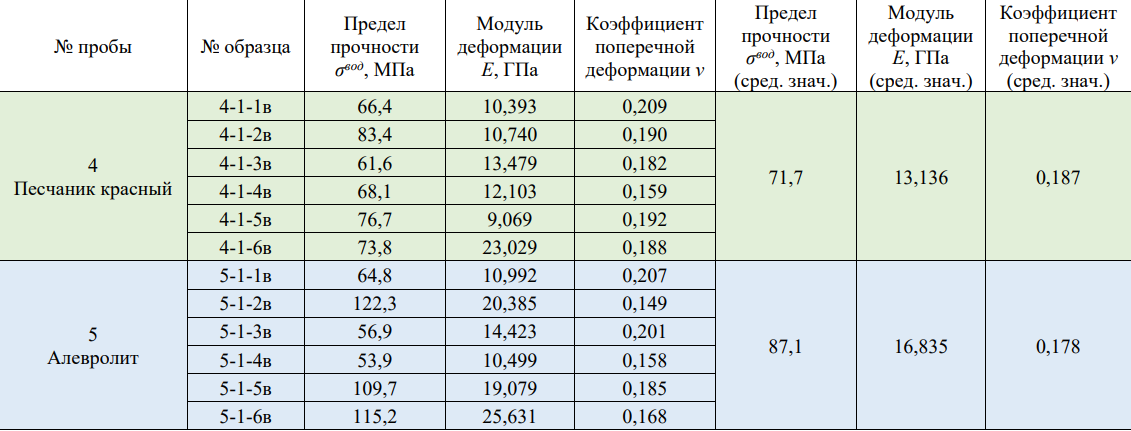
\includegraphics[width=0.9\textwidth]{assets/281}
\end{figure}

\begin{multicols}{2}
При моделировании эти значения были обобщены, изменялся лишь параметр
GSI. Рейтинг GSI является одним из важных параметров, существенно
влияющих на результаты моделирование. В расчетах выполнялись с
применением критерия Хука-Брауна. GSI, представленный Хуком и Брауном в
1994, 1995 и 1998 г.г., представляет собой систему полевого определения
прочности породного массива для различных геологических условий, которая
основана на визуальной оценке структуры массива (блочности) и
характеристик трещин (шероховатость и степень изменения). Сочетание этих
двух параметров позволяет выполнить оценку породного массива, имеющего
различную структуру.

Для обоснования параметров очистной камеры и целиков выполнялся
численное моделирование с изменением ширины камер и МКЦ. Моделирование
выполнялось для углов падение 20, 25, 30 и 35 градусов. В ходе
моделирование определены показатели коэффициента запаса прочности (SF),
а также показатели главных сжимающих (Sigma1) и растягивающих (Sigma3)
напряжений. Определение необходимых участков, таких как зона
концентрации и разгрузки напряжения, осуществляется за счет главных
сжимающих и растягивающих напряжений {[}2{]}.

При проведении горной выработки происходит перераспределение напряжений
в окружающих породах: одни из компонентов тензора напряжений возрастают,
другие уменьшаются. Степень изменения напряжений по сравнению с исходным
их уровнем называется концентрацией и разгрузкой. По стандаратам
международного общества по горной механике (ISRM) для безопасного
ведения горных работ, коэффициент запаса устойчивости горных пород
должен быть выше значение 1,2 {[}3{]}.

Значение 1,2, использованное в рамках исследования, принято на основании
исследования Рида и Стэйси (2009 г.), проведенного в продолжение работ
Суона и Сепульведы (2000 г.). результаты данных исследовании признана
международным обществом по горной механике (ISRM) {[}3{]}.

Для горнотехнических условий разработки Жиландинского месторождения
расположение междукамерных целиков принимается по квадратной сетке с
расстоянием между осями равным 20х20м.

Согласно Технологическому регламенту по применению камерно-столбовой
системы разработки с оставлением столбчатых целиков на подземных
рудниках Жезказганского месторождения {[}4{]}, при отработке наклонных
залежей соблюдать следующие условия расположения междукамерных целиков:

- в диапазоне изменения углов падения залежей 15˚-25˚ междукамерные
целики размещать вертикально;

- в диапазоне изменения углов падения залежей свыше 25˚ до 35˚
междукамерные целики должны быть размещены с наклоном в сторону
восстания на угол β = α/2 (где: α - угол падения залежей) относительно
нормали к напластованию.

{\bfseries Результаты и обсуждения}. На ниже приведенных рисунках
представлены результаты численного моделирования при мощности рудного
тела 5 метров и при углах падения 20-35 градусов. Моделирование
выполнено на основе анализа физико-механических свойств и структурных
особенностей горных пород.

По результатам моделирования, представленные на рисунках 1, 2 и 3 видно,
что при угле падения 20 градусов очистная камера и целики в целом
находятся в устойчивом состоянии. К чему свидетельствует запас прочности
массива горных пород, представленного виде графика на рисунке 5. По
графику видно, что минимальный запас прочности выше значение 1.2, из
которого следует предполагать, что МКЦ и очистная камера находится в
устойчивом состояний. Максимально допустимая ширина очистной камеры
равен 13.0 метров при минимальной мощности МКЦ 7.0 метров.

При ширине камеры 14 метров и мощности МКЦ 6 метров (рис. 4) высота
неустойчивых участков по кровле камеры составляет 2,5 метров, а
разрушение МКЦ достигает до 1,8 метров, из чего следует утверждать, что
риски обрушения горных пород и разрушения МКЦ велики.

При отработке запасов руды при угле падения 20 градусов
камерно-столбовой системой разработки законтурный массив устойчив,
возможны локальные разрушения горных пород до 0,5 метров преимущественно
с кровли выработки виде отслоений и заколов {[}5{]}. МКЦ находится в
устойчивом состояний, к чему свидетельствует запас прочности МКЦ 1,3 и
более.
\end{multicols}

\begin{figure}[H]
	\centering
	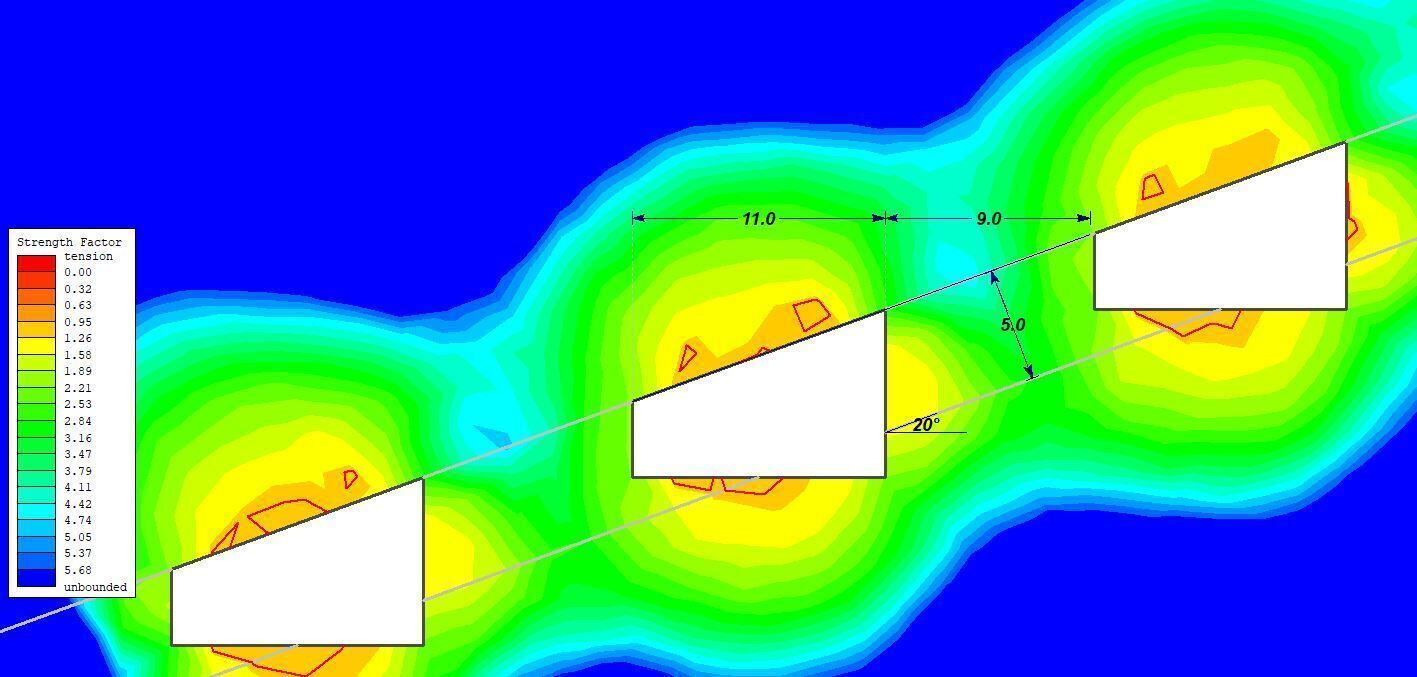
\includegraphics[width=0.6\textwidth]{assets/282}
	\caption*{}
    \caption*{ Рис. 1 - Коэффициент запаса прочности законтурного массива при параметрах очистной камеры 11х9 м и при угле падения 20 градусов}
\end{figure}

\begin{figure}[H]
	\centering
	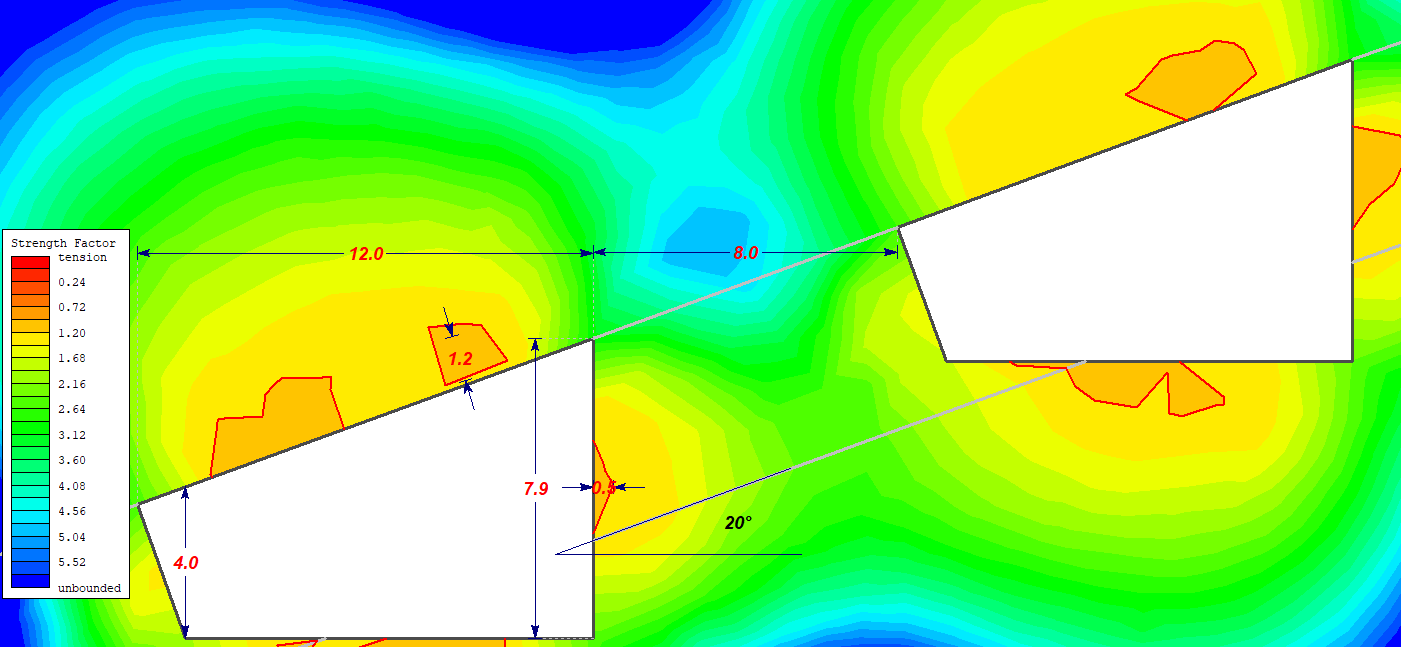
\includegraphics[width=0.6\textwidth]{assets/283}
    \caption*{Рис. 2 - Коэффициент запаса прочности законтурного массива при параметрах очистной камеры 12х8 м и при угле падения 20 градусов}
\end{figure}

\begin{figure}[H]
	\centering
	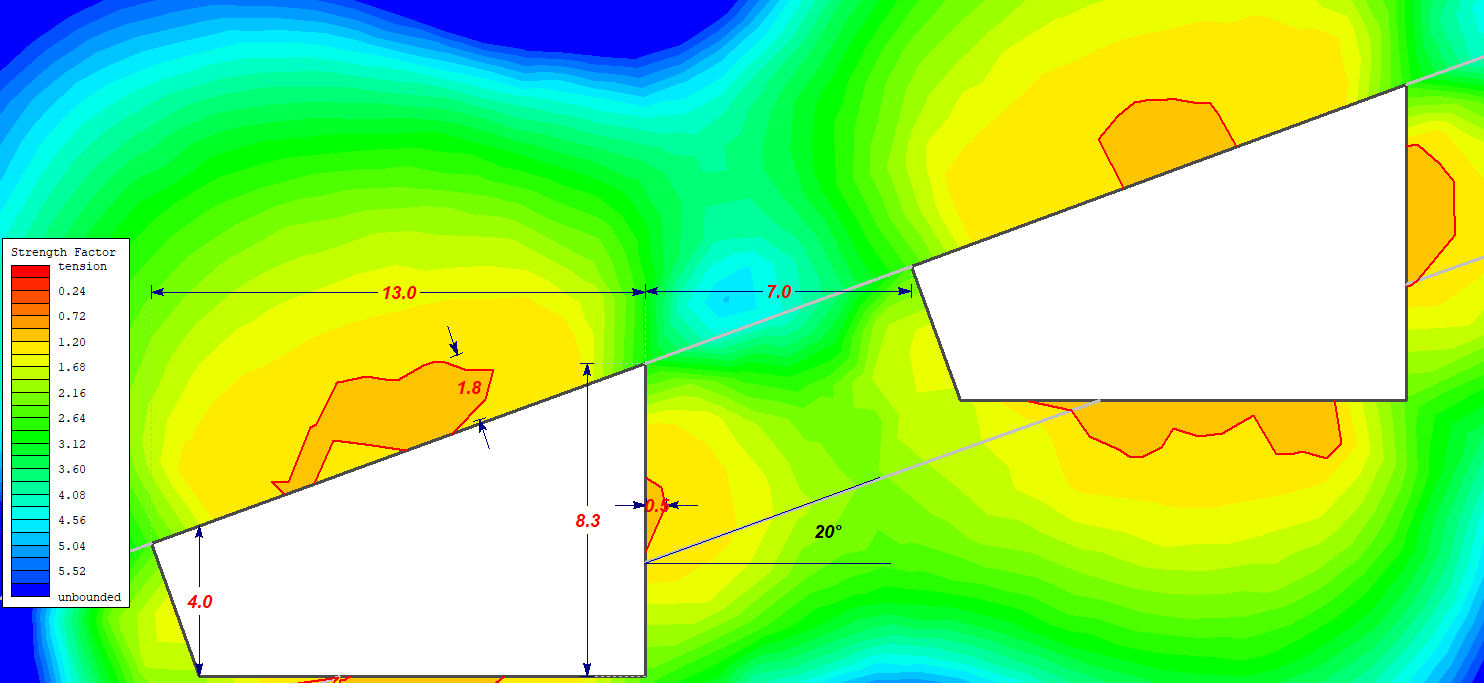
\includegraphics[width=0.6\textwidth]{assets/284}
    \caption*{Рис. 3 - Коэффициент запаса прочности законтурного массива при параметрах очистной камеры 13х7 м и при угле падения 20 градусов}
\end{figure}

\begin{figure}[H]
	\centering
	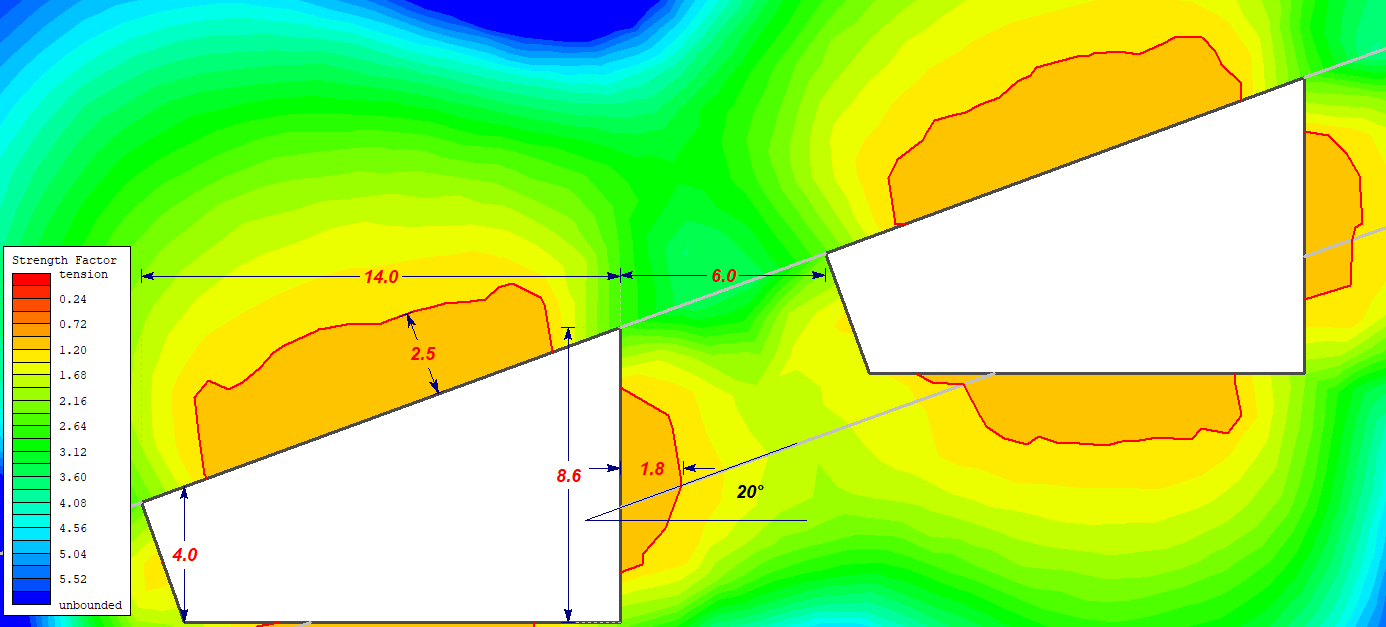
\includegraphics[width=0.6\textwidth]{assets/285}
    \caption*{Рис. 4 - Коэффициент запаса прочности законтурного массива при параметрах очистной камеры 14х6 м и при угле падения 20 градусов}
\end{figure}

\begin{figure}[H]
	\centering
	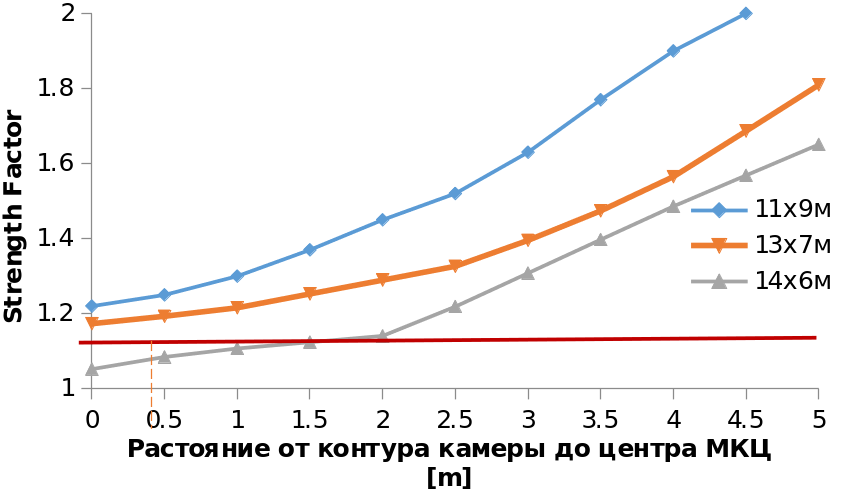
\includegraphics[width=0.7\textwidth]{assets/285.1}
    \caption*{Рис. 5 - Изменение коэффициента запаса прочности МКЦ в зависимости от изменения ширины камеры и мощности МКЦ}
\end{figure}

\begin{figure}[H]
	\centering
	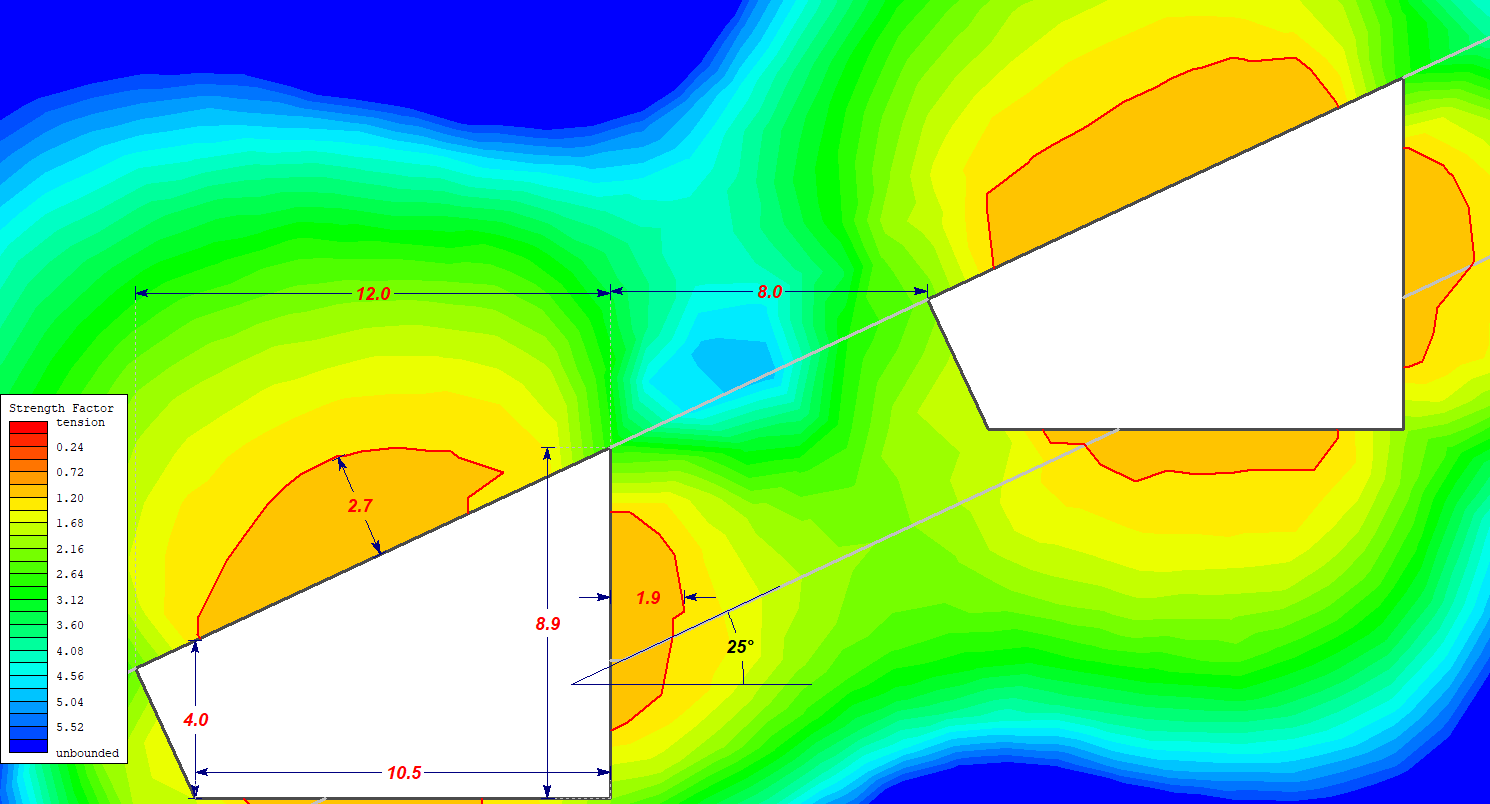
\includegraphics[width=0.6\textwidth]{assets/286}
	\caption*{Рис. 6 - Коэффициент запаса прочности законтурного массива при
параметрах очистной камеры 12х8 м и при угле падения 25 градусов}
\end{figure}

\begin{multicols}{2}
При отработке запасов руды при угле падения 20 градусов не требуется
изменение формы МКЦ на трапециевидную, так как прямые столбчатые МКЦ в
полной мере могут обеспечить устойчивость массива горных пород.

Далее был выполнен моделирование с изменением угла падения до 25
градусов результаты которого приведены на рисунках 6 и 7.

По результатам численного анализа (рис. 6) видно, что при ширине камеры
12 метров и диаметре МКЦ 8 метров коэффициент запаса прочности пород
находятся выше критической отметки равной 1.2. Также результаты
моделирования показал, что возможны обрушения части МКЦ до глубины 1,9
метра, а по кровле очистной камеры зона возможного обрушения доходит до
2,7 метра. В целом МКЦ и очистная камера находится в устойчивом
состоянии.
\end{multicols}

\begin{figure}[H]
	\centering
	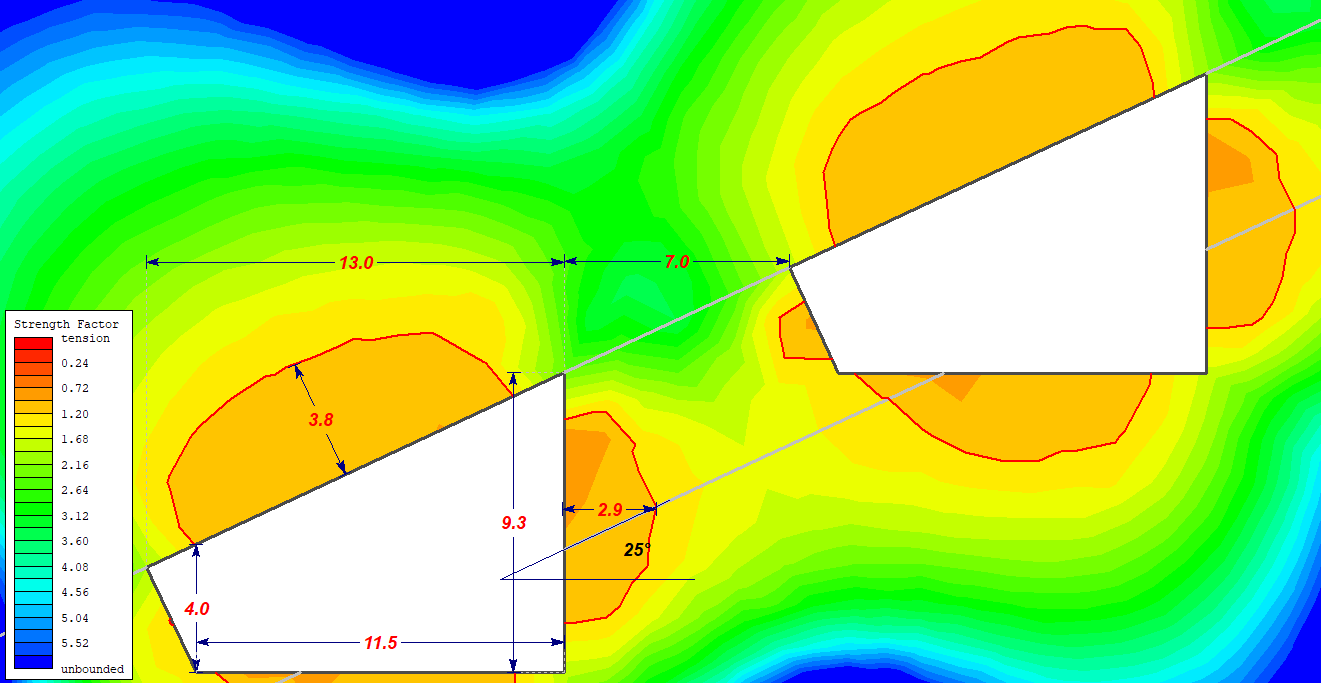
\includegraphics[width=0.6\textwidth]{assets/287}
	\caption*{Рис. 7 - Коэффициент запаса прочности законтурного массива при
параметрах очистной камеры 13х7 м и при угле падения 25 градусов}
\end{figure}

\begin{figure}[H]
	\centering
	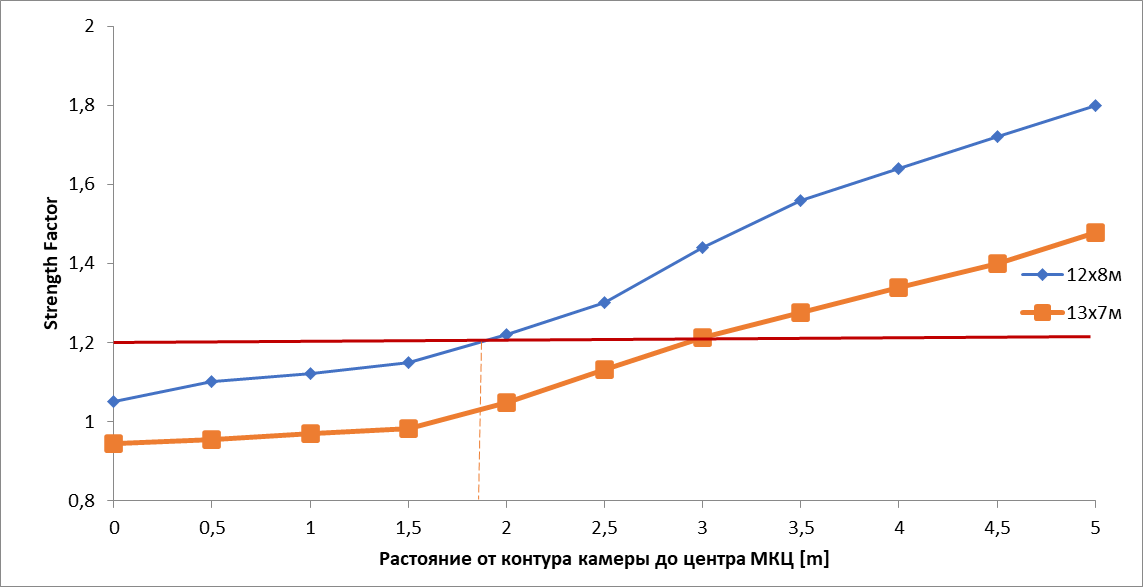
\includegraphics[width=0.6\textwidth]{assets/288}
	\caption*{Рис. 8 - Изменение коэффициента запаса прочности МКЦ}
\end{figure}

\begin{multicols}{2}
На рисунке 7 приведены результаты численного анализа при ширине камеры
13 метров и диаметре МКЦ 7 метров. При таких параметрах по кровле
очистной камеры возможны обрушения до глубины 3,8 метров, а разрушение
МКЦ может достигать до 2,9 метров.

На рисунке 8 приведены изменение коэффициента запаса прочности МКЦ в
зависимости отдаленности от контура камеры.

При угле 25 градусов был выбран трапециевидная форма МКЦ, так как
результаты численного анализа показали, что при столбчатой форме МКЦ
вероятность разрушение МКЦ более высокая. Сравнение результатов
моделирования запаса прочности трапециевидной и прямоугольной МКЦ
диаметром 8 метров приведен на рисунке 9.

Исходя из вышеизложенного следует, что классическая (прямоугольная)
форма МКЦ не эффективен при угле падения рудного тела 25 градусов и
более. Следовательно, при численном анализе массива горных пород при
углах падения рудного тела 30-35 градусов целесообразно принимать
трапециевидную форму МКЦ.

На рисунках 10-11 представлены результаты моделирования при угле 30
градусов. Следует отметить, что при ширине камеры 12 метров и диаметре
МКЦ 8 метров. При таких параметрах по кровле очистной камеры возможны
обрушения до глубины 4,6 метров, а разрушение МКЦ может достигать до 5,3
метров (рис. 10).
\end{multicols}

\begin{figure}[H]
	\centering
	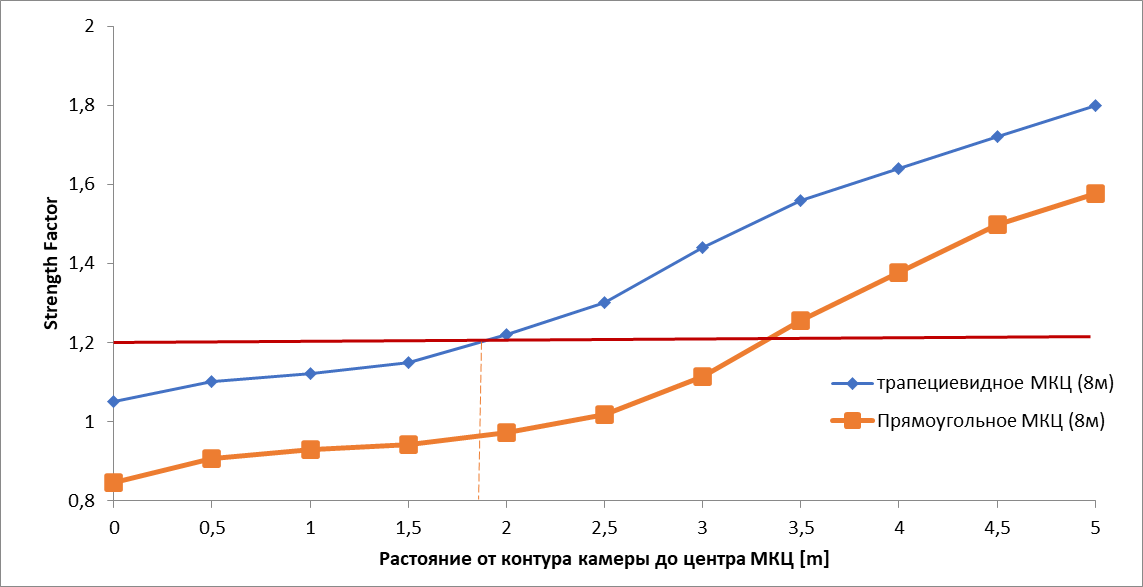
\includegraphics[width=0.6\textwidth]{assets/289}
	\caption*{Рис. 9 - Сравнение трапециевидной и прямоугольной формы МКЦ}
\end{figure}

\begin{figure}[H]
	\centering
	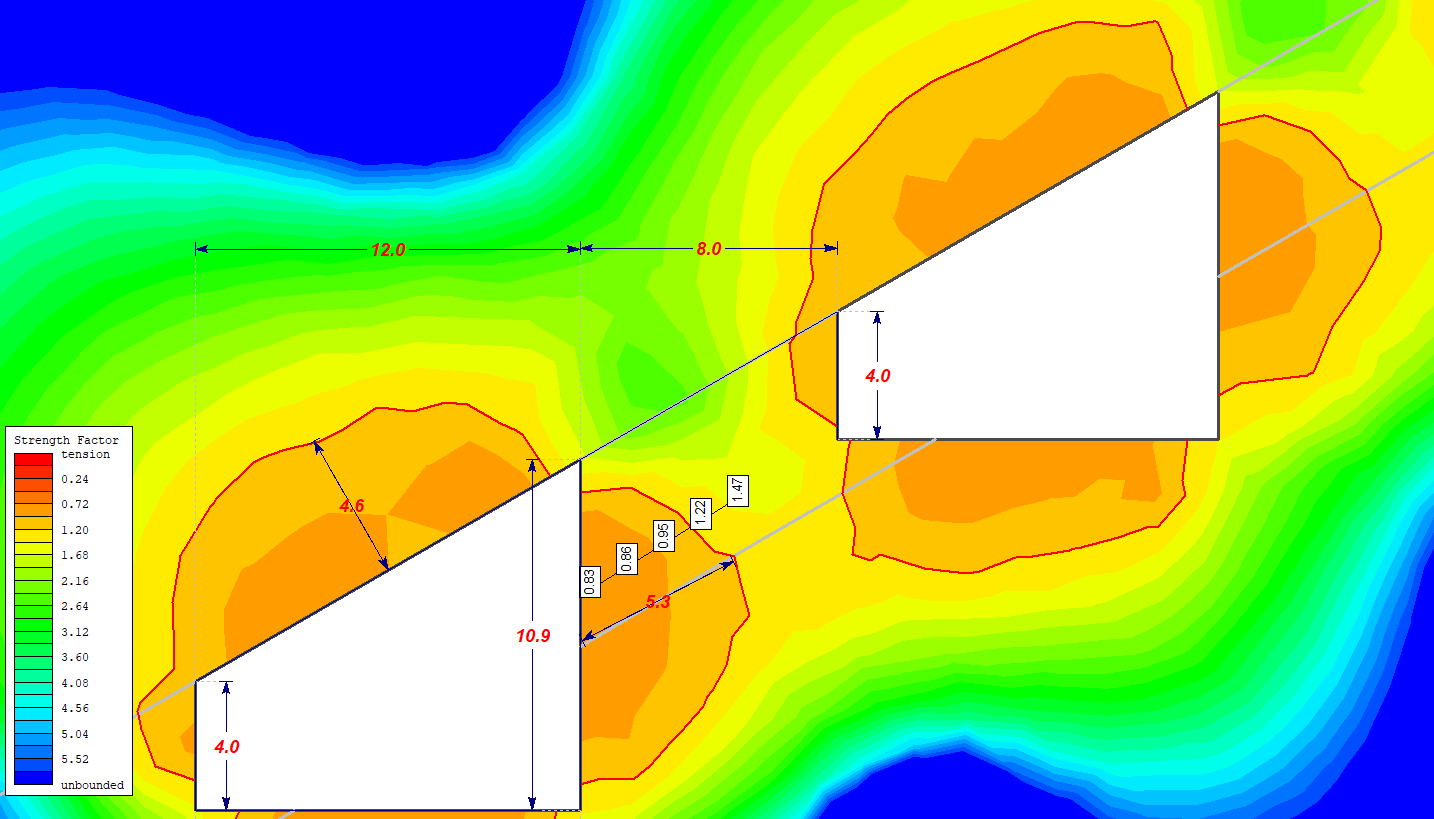
\includegraphics[width=0.6\textwidth]{assets/290}
	\caption*{Рис. 10 - Коэффициент запаса прочности законтурного массива при
параметрах очистной камеры 12х8 м и при угле падения 30 градусов}
\end{figure}

\begin{multicols}{2}
Далее был выполнен численный анализ с изменением формы МКЦ и очистной
камеры на трапециевидную форму {[}6{]}.

Аналогично как на предыдущих моделях был выполнен численный анализ с
изменением ширины камеры на 11 метров, соответственно диаметра МКЦ на 9
метров. На рисунке 11 приведены результаты численного моделирования. По
рисунку видно, что зона возможного обрушения по кровле очистной камеры
не превышает 1,9 метров, тогда как, разрушение МКЦ не превышает 1,8
метра, коэффициент запаса прочности пород больше отметки 1.2, что
говорит об устойчивости МКЦ и камеры.

На рисунке 12 представлена график изменение запасов прочности
классической (12х8 м) и трапециевидной (11х9 м) формы МКЦ, по которому
следует, что при классической форме возможная глубина разрушения может
достигать более 5 метров, тогда как при трапециевидном МКЦ данный
показатель не более 1,8 метров.
\end{multicols}

\begin{figure}[H]
	\centering
	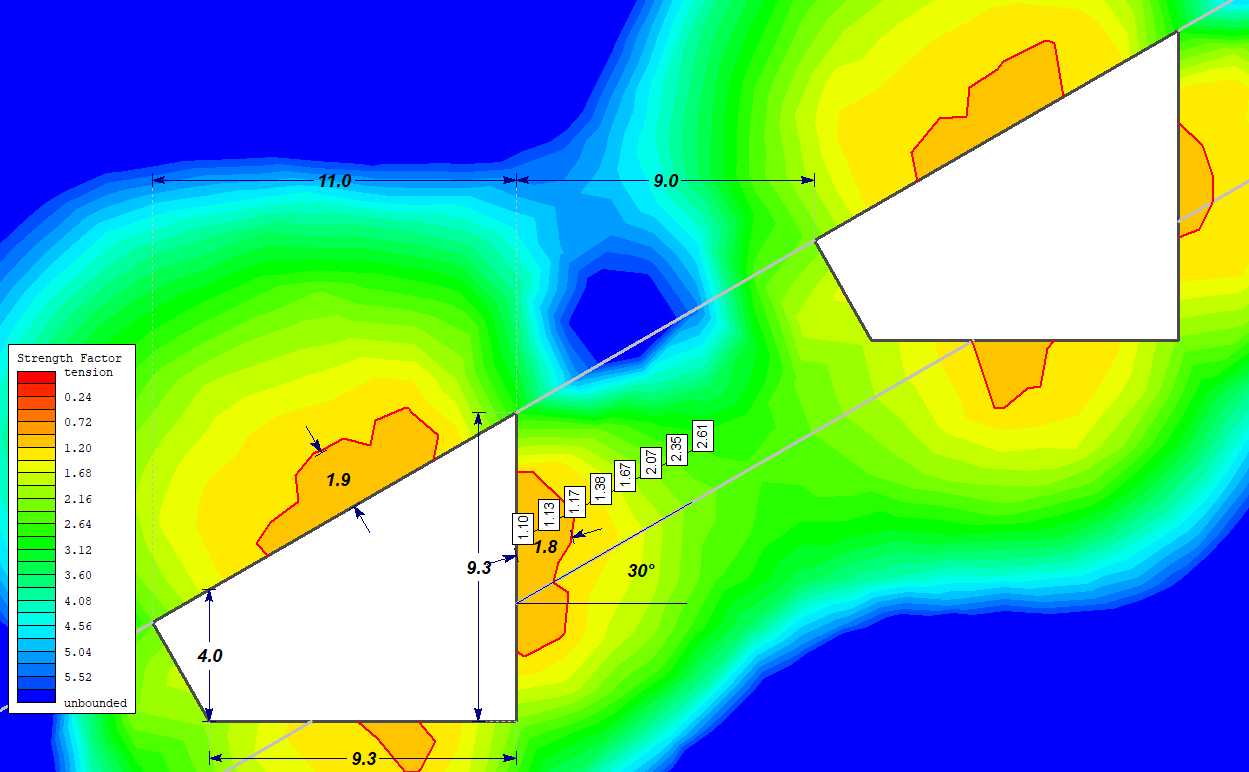
\includegraphics[width=0.65\textwidth]{assets/291}
	\caption*{Рис. 11 - Коэффициент запаса прочности законтурного массива при
параметрах очистной камеры 11х9 м и при угле падения 30 градусов}
\end{figure}

\begin{figure}[H]
	\centering
	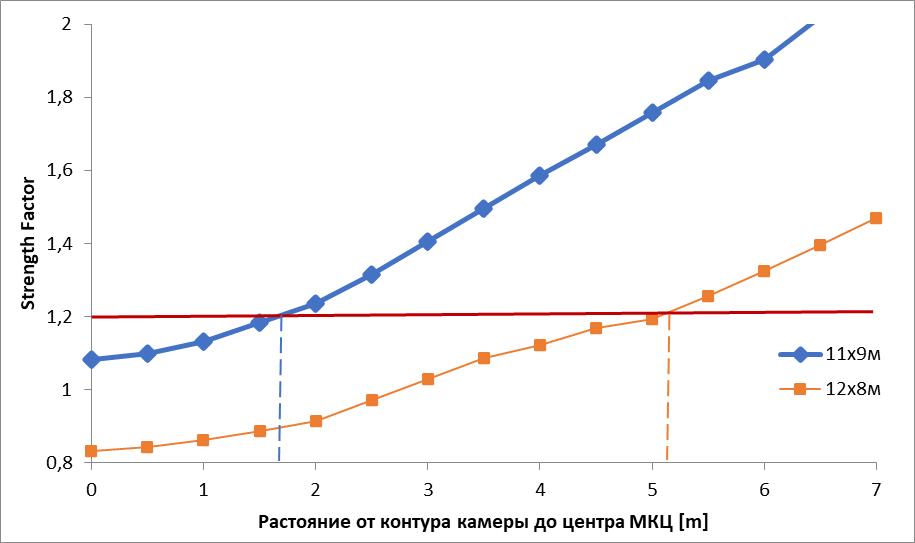
\includegraphics[width=0.65\textwidth]{assets/292}
	\caption*{Рис. 12 - Изменение коэффициента запаса прочности МКЦ}
\end{figure}

На рисунках 13-14 представлены результаты численного моделирования
массива горных пород при угле падения залежей 35 градусов.

\begin{figure}[H]
	\centering
	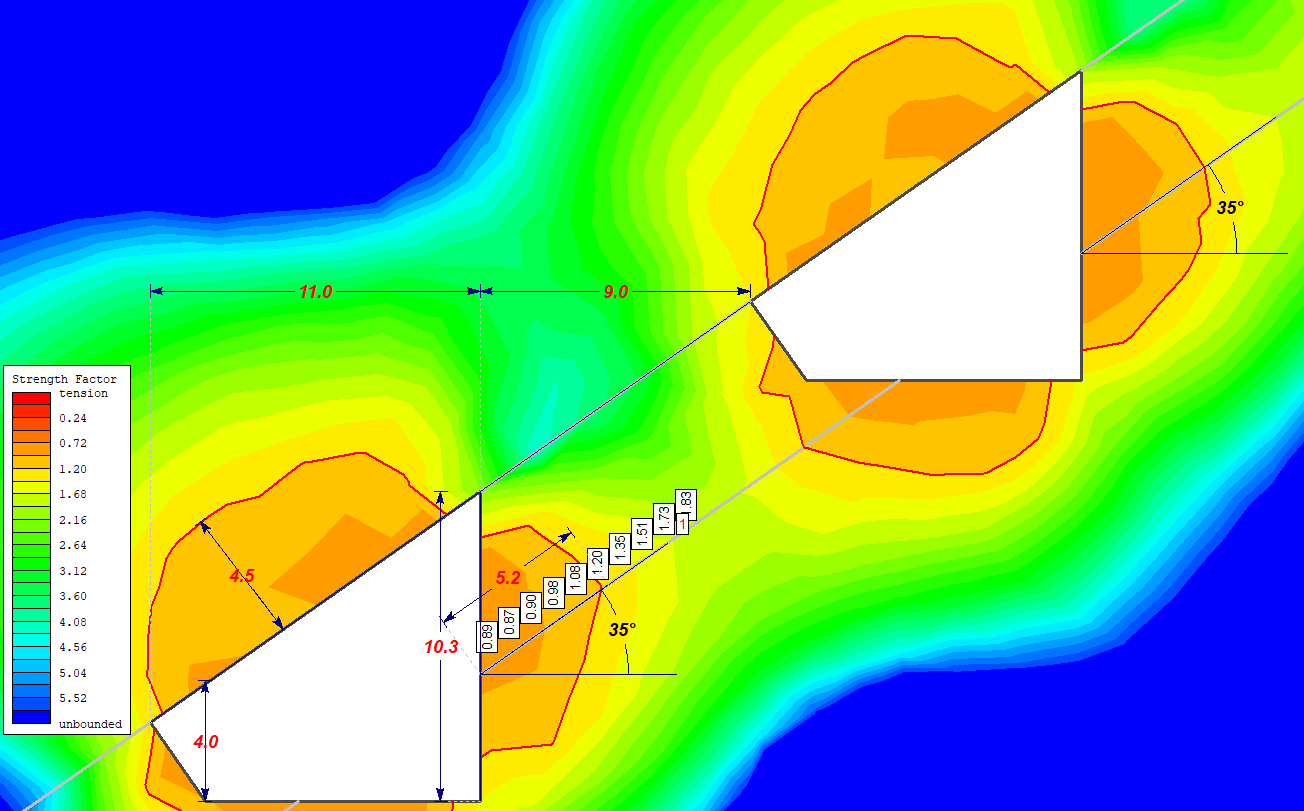
\includegraphics[width=0.65\textwidth]{assets/293}
	\caption*{Рис. 13 - Коэффициент запаса прочности законтурного массива при
параметрах очистной камеры 11х9 м и при угле падения 35 градусов}
\end{figure}

\begin{multicols}{2}
По результатам численного моделирования при угле падения горных пород 35
градусов коэффициент запаса прочности МКЦ трапециевидной формы мощностью
9 метров и при ширине очистной камеры 11 метров (рис. 13) разрушение МКЦ
могут достигать до 5,2 метров, а обрушение кровли могут достигать до 4,5
метров, что ниже допустимых значений. Из чего следует предполагать, МКЦ
не устойчив и вероятность разрушения весьма велика {[}7{]}.

На рисунке 14 представлены результаты моделирования при параметрах
очистной камеры и МКЦ 10х10 м. В данном случае разрушение МКЦ не
превышает 2,2 метра, а обрушение горных пород по кровле не превышает 1,7
метров.

Для более детального сравнение результатов численного моделирования
выполненных методами конечных элементов построена график сравнение
коэффициента запаса прочности, представленного на рисунке 15.
\end{multicols}

\begin{figure}[H]
	\centering
	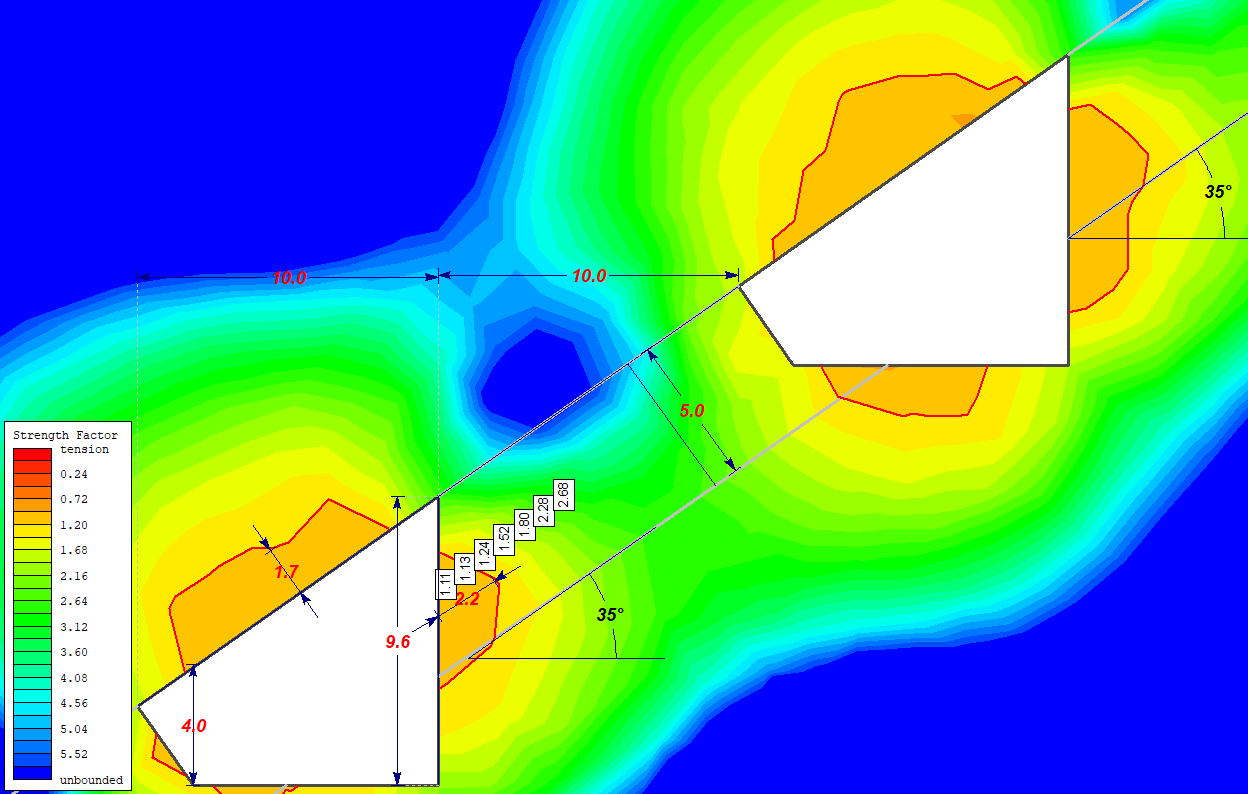
\includegraphics[width=0.65\textwidth]{assets/294}
	\caption*{Рис. 14 - Коэффициент запаса прочности законтурного массива при
параметрах очистной камеры 10х10 м и при угле падения 35 градусов}
\end{figure}

\begin{figure}[H]
	\centering
	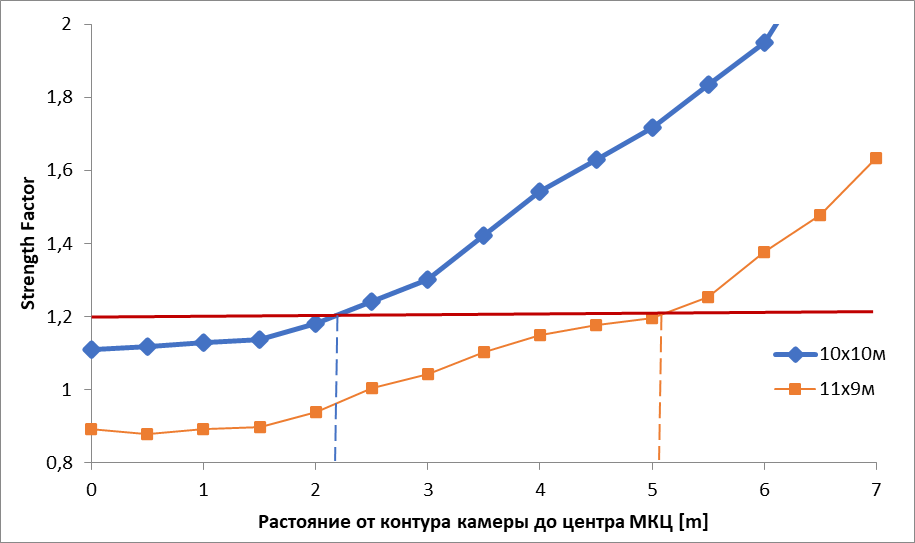
\includegraphics[width=0.65\textwidth]{assets/295}
	\caption*{Рис. 15 - Изменение коэффициента запаса прочности МКЦ}
\end{figure}

В соответствии анализа результатов численного моделирования массива
горных пород методом конечных элементов построены несколько графиков
зависимости, первый из которых приведен на рисунке 16.

\begin{figure}[H]
	\centering
	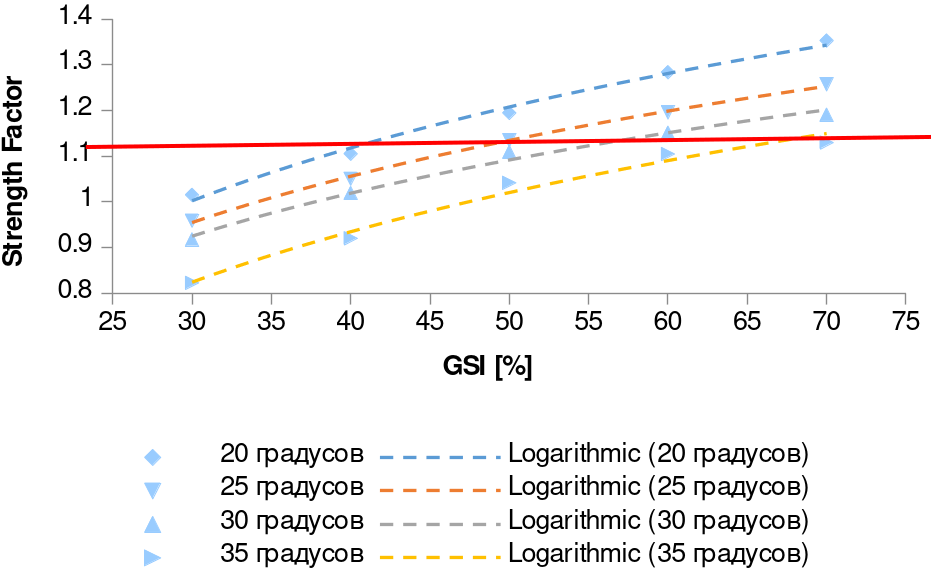
\includegraphics[width=0.7\textwidth]{assets/295.1}
	\caption*{Рис. 16 - График зависимости запаса прочности от GSI и угла падения (при прямоугольной форме МКЦ)}
\end{figure}

\begin{multicols}{2}
Данный график наглядно показывает, что МКЦ прямоугольной формы допустима
только в случае, если угол падения 20 градусов и GSI не менее 50 \%, в
остальных случаях горный массив не устойчив и вероятность обрушения МКЦ
весьма велика.

На следующем рисунке 17 представлены аналогичный график зависимости,
только для трапециевидной формы МКЦ мощностью 10 метров. Данный график
построен на основе интерпретации данных численного анализа МКЭ. Был
выполнен анализ с различными вариантами GSI.
\end{multicols}

\begin{figure}[H]
	\centering
	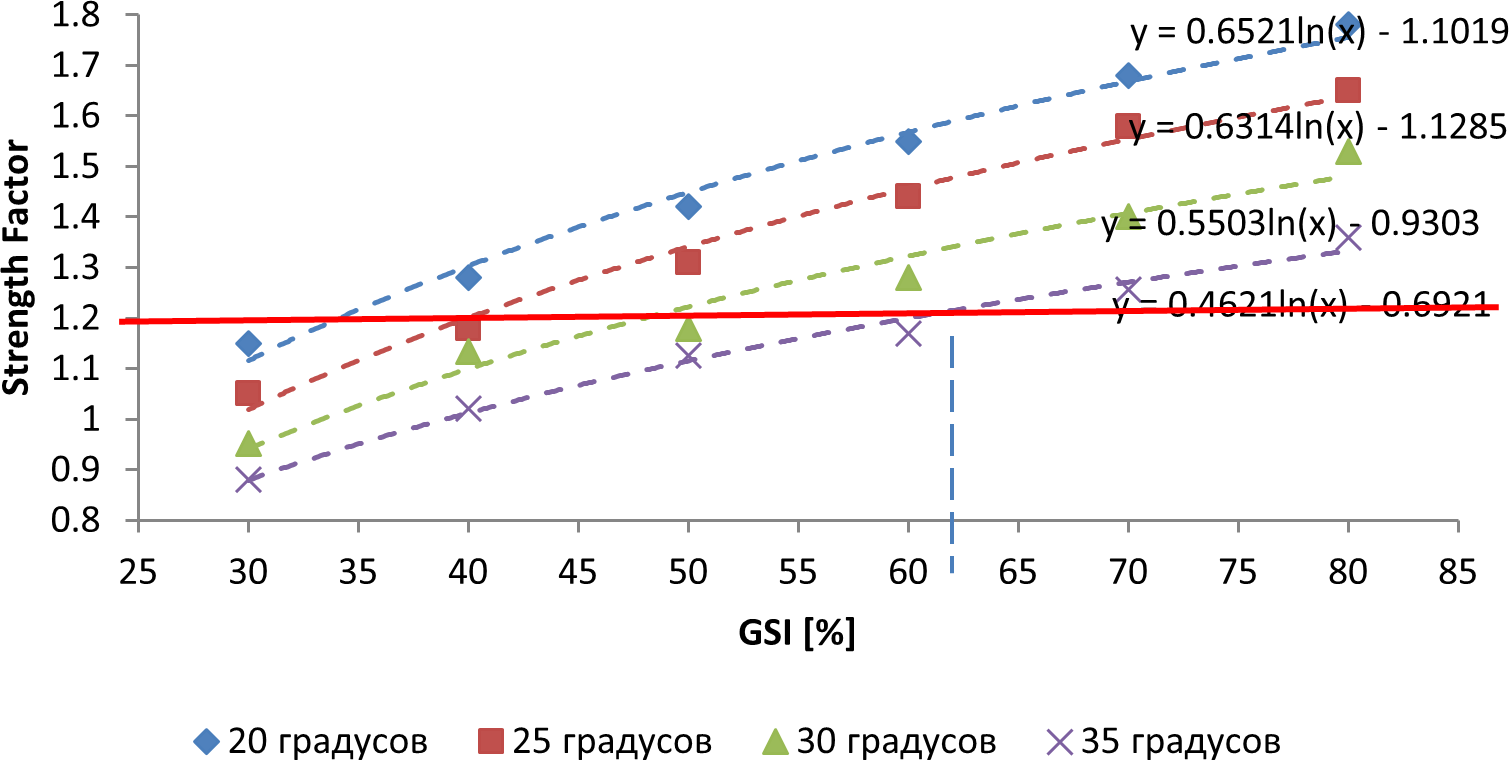
\includegraphics[width=0.7\textwidth]{assets/295.2}
	\caption*{Рис. 17 - График зависимости запаса прочности от GSI и угла падения (при трапециевидной форме МКЦ)}
\end{figure}

\begin{multicols}{2}
По полученным результатам видно, что коэффициент запаса прочности (SF)
напрямую зависит от рейтинга массива GSI и угла падения залежей {[}8{]}.

По графику видно, что трапециевидное форма МКЦ в целом обеспечивает
сохранность выработанного пространства и целиков при углах падения:

20 градусов - обеспечивает сохранность МКЦ и камеры при GSI не менее
35\%;

25 градусов - обеспечивает сохранность МКЦ и камеры при GSI не менее
40\%;

30 градусов - обеспечивает сохранность МКЦ и камеры при GSI не менее
50\%;

35 градусов - обеспечивает сохранность МКЦ и камеры при GSI не менее
63\%.

{\bfseries Выводы.} Для обоснования допустимых параметров очистных камер и
целиков был выполнен анализ данных полученных в результате численного
моделирования массива горных пород. На основе комплекса выполненных
исследовании определены допустимые параметры очистной камеры и
междукамерного целика в зависимости от угла залегания.

На основе численного моделирования массива горных пород углом падения
20-35 градусов методами конечных элементов в программе RS-2 и в
результате дальнейшего анализа полученных данных о
напряженно-деформационного состояния были построены графики зависимости
позволяющие определять коэффициент запаса прочности (Strength Factor) в
зависимости от геологического индекса прочности (GSI) {[}9{]}.

Результаты моделирования показывает, что МКЦ классической (вертикальной)
формы мощностью 7 метров допустим только в случае, если угол падения
рудного тела 20-25 градусов и GSI не менее 50 \%, в остальных случаях
горный массив не устойчив и вероятность обрушения МКЦ {[}10{]} весьма
велика.

По результатам моделирования напряженного состояния следует, что в
окружающих выработку породах возникает зоны концентрация и разгрузки
напряжений. Она довольно быстро убывает вглубь массива, и на расстоянии
5-7 полупролетов выработки напряжения практически не отличаются от тех,
что действовали в массиве до проведения выработки.

\emph{{\bfseries Финансирование:} Научно-исследовательская работа выполнена
в рамках ГФ Министерством науки и высшего образования Республики
Казахстан №AP 19677938 по теме «Создание метода прогнозирования
сдвижения вмещающих пород до земной поверхности для модернизации
технологии повторной разработки пологих рудных залежей» на 2023-2025 гг.
Авторский коллектив также выражает благодарность руководству ТОО
«Корпорация Казахмыс» за предоставленную возможность проведения
исследовательских работ на базе предприятия. Особую благодарность
следует выразить редакторам и рецензентам журнала за их ценные советы,
которые были учтены для улучшения качества публикации.}
\end{multicols}

\begin{center}
{\bfseries Литература}
\end{center}

\begin{noparindent}
1. Отчет о научно-исследовательской работе: Геомеханическое обоснование
отработки месторождений Жиландинской группы {[}док.внутреннего
пользования{]} / ТОО «Expert PRO». - Сатпаев-Усть-Каменогорск, 2022 .

2. Shichuan Zhang, Yangyang Li, Baotang Shen, Xizhen Sun, Liqun Gao.
Effective evaluation of pressure relief drilling for reducing rock
bursts and its application in underground coal mines // International
Journal of Rock Mechanics and Mining Sciences.). -2019. Vol. 114(11).
-P. 7-16. DOI 10.1016/j.ijrmms.2018.12.010

3. Read John \& Stacey Peter. Guidelines for Open Pit Slope Design. -
2009. DOI 10.1071/9780643101104

4. Технологическая инструкция по применению камерно-столбовой системы
разработки {[}док.внутреннего пользования{]} /ТОО «Корпорация Казахмыс».
- Жезказган, 2017.

5. Zhienbayev, A., Zharaspaev, M., Balpanova, M., Nurkasyn, N., Asanova,
Z., Zhakupov, B. Analysis of the roof span stabil-ity in terms of
room-and-pillar system of ore deposit mining// Mining of Mineral
Deposits. - 2023. Vol. 17(1). - P. 129-137. DOI
10.33271/mining17.01.129

6. Mahdevari, Satar \& Shahriar, Kourosh \& Sharifzadeh, Mostafa \&
Tannant, Dwayne. (2017). Stability prediction of gate roadways in
longwall mining using artificial neural networks // Neural Computing and
Applications. -2016. -Vol. 28. -P. 3537-3555. DOI
10.1007/s00521-016-2263-2

7. Fitsak V.V., Lomakina E.S., Strakhova A.A. and Chernobai V.I.
Determination of Room-and-Pillar system parameters for Transition to
Greater Depths// International Journal of Applied Engineering Research.
- 2017. - Vol. 12(22). -P. 12322-12331.

8. Ivadilinova, D. \& Issabek, T. \& Takhanov, D. \& Yeskenova, Gulnura.
Predicting underground mining impact on the earth's sur-face // Naukovyi
Visnyk Natsionalnoho Hirnychoho Universytetu. -2023. -P. 32-37. DOI
10.33271/nvngu/2023-1/032

9. Félix Del Pozo, Eduardo Córdova, Carlos Marquardt, Rodolfo Cabezas G,
Philip Benson, Nick Koor, John Browning, Rocío Rudloff, Development of a
geomechanical model based on suitable estimations of GSI and UCS in
mining production slopes at the TilTil district, central Chile //
International Journal of Rock Mechanics and Mining Sciences. - 2023. -
Vol. 167(3). DOI 10.1016/j.ijrmms.2023.105390

10. Serebryakov E.V., Gladkov A.S. Geological and structural
characteristics of deep-level rock mass of the Udachnaya pipe deposit //
Journal of Mining Institute. - 2021. - Vol. 250. - P. 512-525. DOI
10.31897/PMI.2021.4.4
\end{noparindent}

\begin{center}
{\bfseries References}
\end{center}

\begin{noparindent}
1. Otchet o nauchno-issledovatel\textquotesingle skoi rabote:
Geomekhanicheskoe obosnovanie otrabotki mestorozhdenii Zhilandinskoi
gruppy {[}dok.vnutrennego pol\textquotesingle zovaniya{]} / TOO «Expert
PRO». - Satpaev-Ust\textquotesingle-Kamenogorsk, 2022.

2. Shichuan Zhang, Yangyang Li, Baotang Shen, Xizhen Sun, Liqun Gao.
Effective evaluation of pressure relief drilling for reducing rock
bursts and its application in underground coal mines // International
Journal of Rock Mechanics and Mining Sciences.). -2019. Vol. 114(11).
-P. 7-16. DOI 10.1016/j.ijrmms.2018.12.010

3. Read John \& Stacey Peter. Guidelines for Open Pit Slope Design. -
2009. DOI 10.1071/9780643101104

4. Tekhnologicheskaya instruktsiya po primeneniyu kamerno-stolbovoi
sistemy razrabotki {[}dok.vnutrennego pol\textquotesingle zovaniya{]}
/TOO «Korporatsiya Kazakhmys». - Zhezkazgan, 2017.

5. Zhienbayev, A., Zharaspaev, M., Balpanova, M., Nurkasyn, N., Asanova,
Z., Zhakupov, B. Analysis of the roof span stabil-ity in terms of
room-and-pillar system of ore deposit mining// Mining of Mineral
Deposits. - 2023. Vol. 17(1). - P. 129-137. DOI
10.33271/mining17.01.129

6. Mahdevari, Satar \& Shahriar, Kourosh \& Sharifzadeh, Mostafa \&
Tannant, Dwayne. (2017). Stability prediction of gate roadways in
longwall mining using artificial neural networks // Neural Computing and
Applications. -2016. -Vol. 28. -P. 3537-3555. DOI
10.1007/s00521-016-2263-2

7. Fitsak V.V., Lomakina E.S., Strakhova A.A. and Chernobai V.I.
Determination of Room-and-Pillar system parameters for Transition to
Greater Depths// International Journal of Applied Engineering Research.
- 2017. - Vol. 12(22). -P. 12322-12331.

8. Ivadilinova, D. \& Issabek, T. \& Takhanov, D. \& Yeskenova, Gulnura.
Predicting underground mining impact on the earth's sur-face // Naukovyi
Visnyk Natsionalnoho Hirnychoho Universytetu. -2023. -P. 32-37. DOI
10.33271/nvngu/2023-1/032

9. Félix Del Pozo, Eduardo Córdova, Carlos Marquardt, Rodolfo Cabezas G,
Philip Benson, Nick Koor, John Browning, Rocío Rudloff, Development of a
geomechanical model based on suitable estimations of GSI and UCS in
mining production slopes at the TilTil district, central Chile //
International Journal of Rock Mechanics and Mining Sciences. - 2023. -
Vol. 167(3). DOI 10.1016/j.ijrmms.2023.105390

10. Serebryakov E.V., Gladkov A.S. Geological and structural
characteristics of deep-level rock mass of the Udachnaya pipe deposit //
Journal of Mining Institute. - 2021. - Vol. 250. - P. 512-525. DOI
10.31897/PMI.2021.4.4
\end{noparindent}

\emph{{\bfseries Information about the authors}}

\begin{noparindent}
D.K. Takhanov - Candidate of Technical Sciences, Karaganda Technical
University named after Abylkas Saginov, Karaganda, Kazakhstan, e-mail:
takhanov80@mail.ru;

Balpanova M.J. - PhD, Karaganda Technical University named after Abylkas
Saginov, Karaganda, Kazakhstan, e-mail: balpanova86@mail.ru;

Ivadilinova D.T. - PhD, Karaganda Technical University named after
Abylkas Saginov, Karaganda, Kazakhstan, e-mail: dinulb@mail.ru.
\end{noparindent}

\emph{{\bfseries Сведения об авторах}}

\begin{noparindent}
Таханов Д.К. - кандидат технических наук, Карагандинский технический
университет имени Абылкаса Сагинова, Караганда, Казахстан, e-mail:
takhanov80@mail.ru;

Балпанова М.Ж. - доктор PhD, Карагандинский технический университет
имени Абылкаса Сагинова, Караганда, Казахстан, e-mail:
balpanova86@mail.ru;

Ивадилинова Д.Т. - доктор PhD, Карагандинский технический университет
имени Абылкаса Сагинова, Караганда, Казахстан, e-mail: dinulb@mail.ru.
\end{noparindent}




